\documentclass[11pt]{scrartcl}
\usepackage[utf8]{inputenc} % Kodierung der Textdatei mit Sonderzeichen
\usepackage[ngerman]{babel} % Sprache fuer Inhaltsverzeichnis etc.
\usepackage{amssymb} % Mathematische Symbole
\usepackage{amsmath} % Mehr mathematische Konstrukte
\usepackage{graphicx} % Um Bilder einbinden zu koennen
\usepackage{float} % fuer \begin{figure}[H]
\usepackage{icomma} % laesst das Komma als Dezimaltrennzeichen interpretieren
\usepackage{fix-cm} % für die große Titelschrift
\usepackage[pdftex]{hyperref} % Hyperlinks im Dokument
\hypersetup{colorlinks=true, linkcolor=black, citecolor=black, filecolor=black, urlcolor=black, pdftitle={LED-Spektrometer - Projektpraktikum 09/10 Gruppe 5}}


\newcommand{\unit}[1]{\ensuremath{\,\mathrm{#1}}} % Einheiten schreiben sich immer aufrecht!
\newcommand{\degr}{\ensuremath{^\circ}}
\newcommand{\cel}{\ensuremath{\degr\mathrm{C}}}
\newcommand{\dif}{\ensuremath{\mathrm{d}}}
\newcommand{\pdif}[2]{\ensuremath{\frac{\partial#1}{\partial#2}}}
\newcommand{\ee}[1]{\ensuremath{\cdot 10^{#1}}}
\newcommand{\hypref}[2]{\hyperref[#2]{{#1}~\ref{#2}}}

\setlength{\parindent}{1em}
\setlength{\parskip}{0.5\baselineskip}


\title{LED-Spektrometer - Gruppe 5 WS 09/10, Projektpraktikum der Uni Erlangen}
\date{07.12.2009 -- 15.01.2010}
\author{Michele Collodo, Andreas Glossner, Karl-Christoph G\"odel, Bastian Hacker, Maria Obst, Alexander Wagner, David Winnekens}



\begin{document}
\sloppy % laesst Latex nicht ueber den Rand rausschreiben
\thispagestyle{empty}
\large{Projektpraktikum WS 09/10}
\hfill
\raisebox{-1.4cm}{
\includegraphics[width=5cm]{images/fau.pdf}}
\\[8\baselineskip]
\begin{center}
{\fontsize{36}{54}\textbf{LED-Spektrometer}}
\\[2\baselineskip]
{\Large 07.12.2009 -- 15.01.2010}
\\[7\baselineskip]
{\huge\textbf{PPG 5}}
\\[0.5\baselineskip]
{\large\textbf{
Michele Collodo,
Andreas Glossner,\\
Karl-Christoph G\"odel,
Bastian Hacker,\\
Maria Obst,
Alexander Wagner,
David Winnekens}\\
Tutor: Xiaoyue Jin}
\vfill



\small{\url{http://pp.physik.uni-erlangen.de/groups/ws0910/ppg5/ppg5\_start.html}}
\end{center}
\newpage



\tableofcontents
\vfill



\begin{abstract}
Bla
\end{abstract}
\newpage


\section{Grundgedanke des Versuchs}

\subsection{Aufbau und Funktionsweise einer LED}
Die Leuchtdiode, kurz LED (für engl. "Light Emitting Diode") ist eine Halbleiter-Diode die es ermöglicht elektrische Energie in Licht verschiedener Wellenlängen umzuwandeln.

Da im vorliegenden Projekt nur bedrahtete LEDs als Absorber verwendet wurden, wird im Folgenden nur der Aufbau dieser Leuchtdioden-Bauform dargestellt. Die prinzipielle Funktionsweise ist jedoch bei fast allen Bauarten identisch. Lässt man durch Anode und Kathode der LED einen Strom in Durchlassrichtung fließen, so beginnt der Halbleiter in einer von Material und Dotierung abhängigen Wellenlänge zu strahlen. Für Leuchtdioden im sichtbaren Spektralbereich, wie sie hier verwendet wurden, kommt meist eine Galliumverbindung zum Einsatz.

\begin{figure}[ht]
\begin{center}
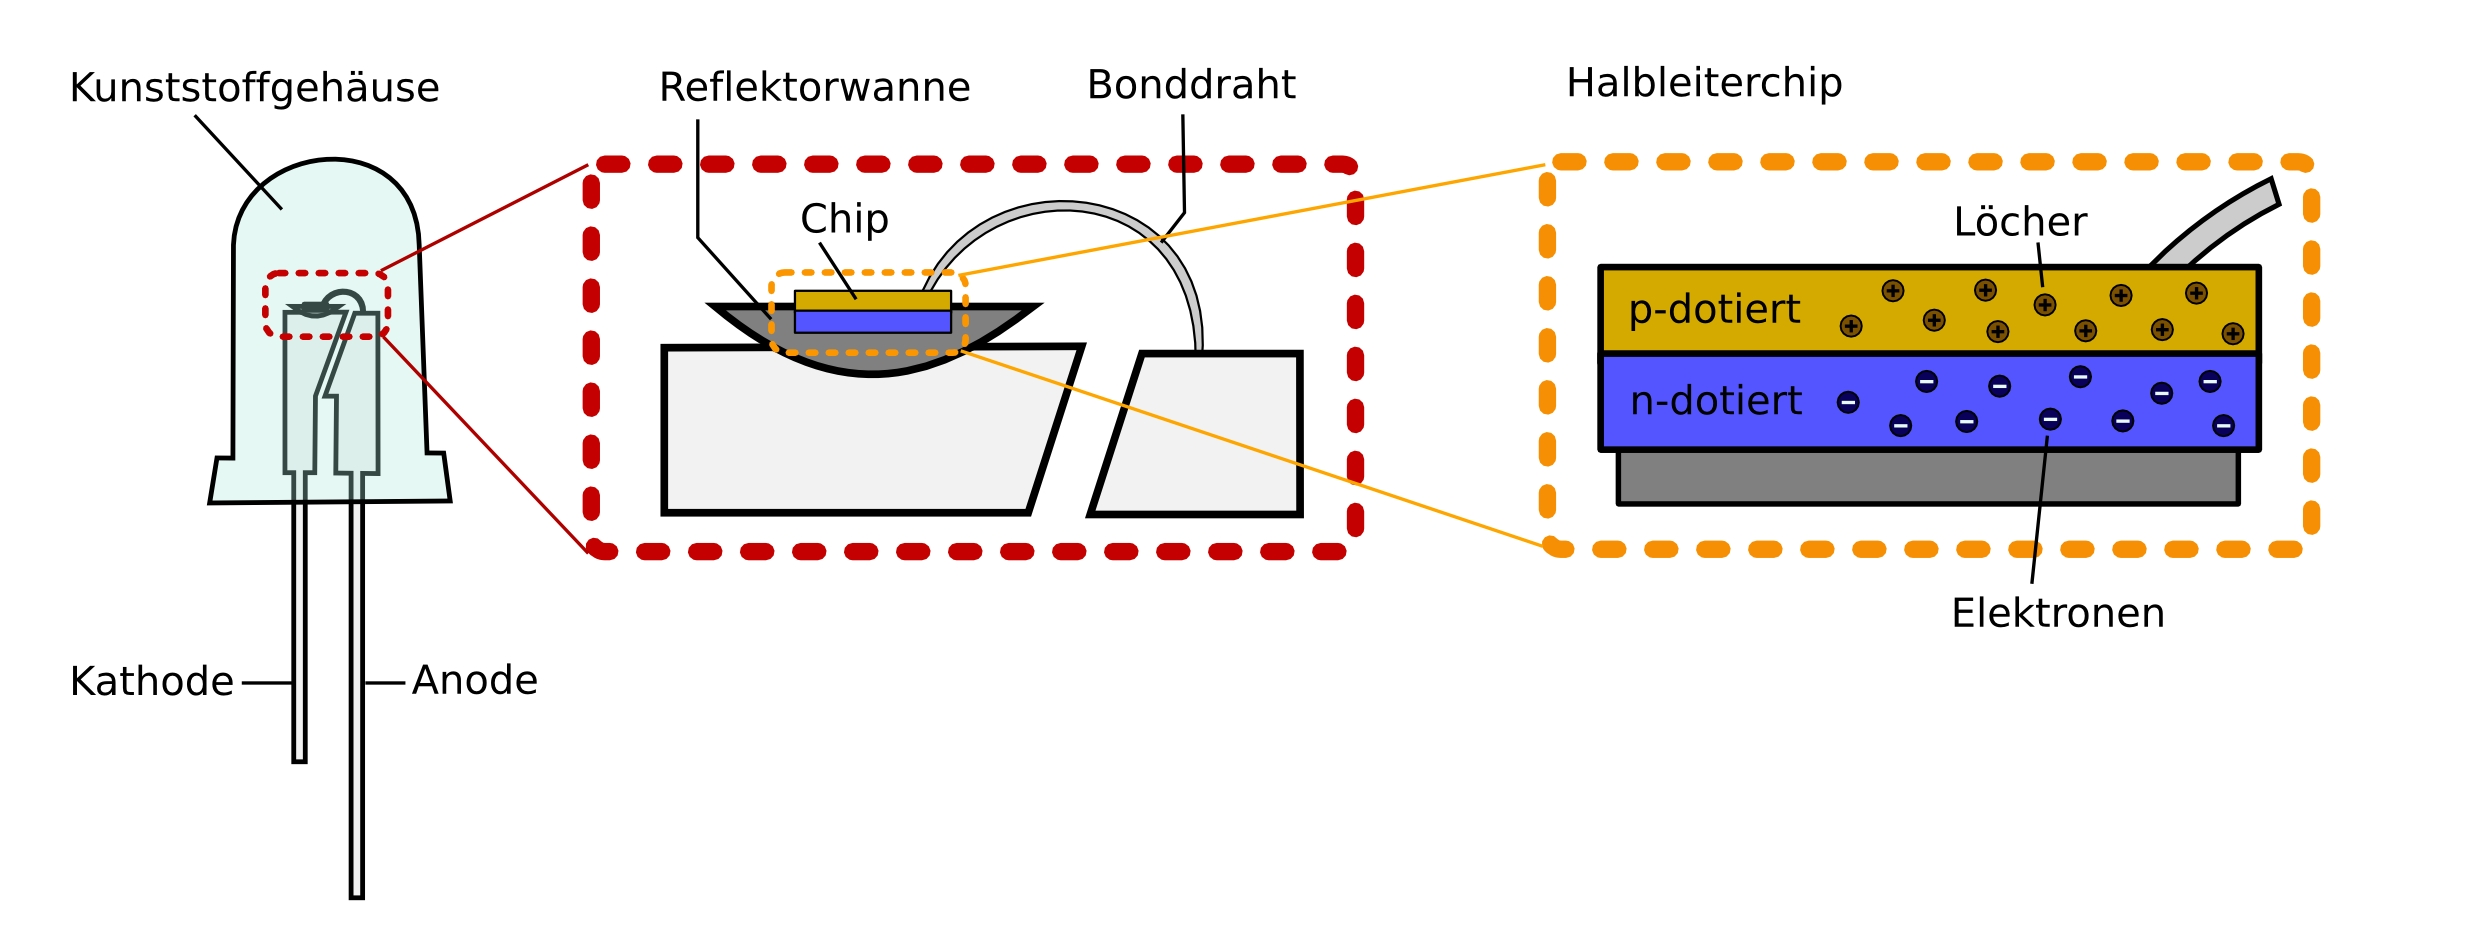
\includegraphics[width=0.8\textwidth]{images/ledaufbau.jpg}
\end{center}
\vspace{-1.5\baselineskip}
\caption{Aufbau einer bedrahteten Leuchtdiode}
\label{LED-Aufbau}
\end{figure}

Das Funktionsprinzip einer LED basiert auf dem Aufbau des Chips, der aus zwei verschieden dotierten Halbleiterschichten besteht. In der p-dotierten Schicht befindet sich ein Überschuss an positiven Ladungsträgern (Löcher), in der n-dotierten Schicht überwiegen negativ geladenen Teilchen (Elektronen). Wird nun ein Strom in Durchlassrichtung an den Chip angelegt, können Elektronen und Löcher am p-n-Übergang rekombinieren. Da sich die Elektronen im n-dotierten Halbleiter im Leitungsband befinden und auf das energetisch niedriger liegende Valenzband der p-dotierten Schicht wechseln, wo sie mit den Löchern rekombinieren, wird ein fester Energiebetrag frei, der in Form eines Photons abgestrahlt wird.

\begin{figure}[ht]
\begin{center}
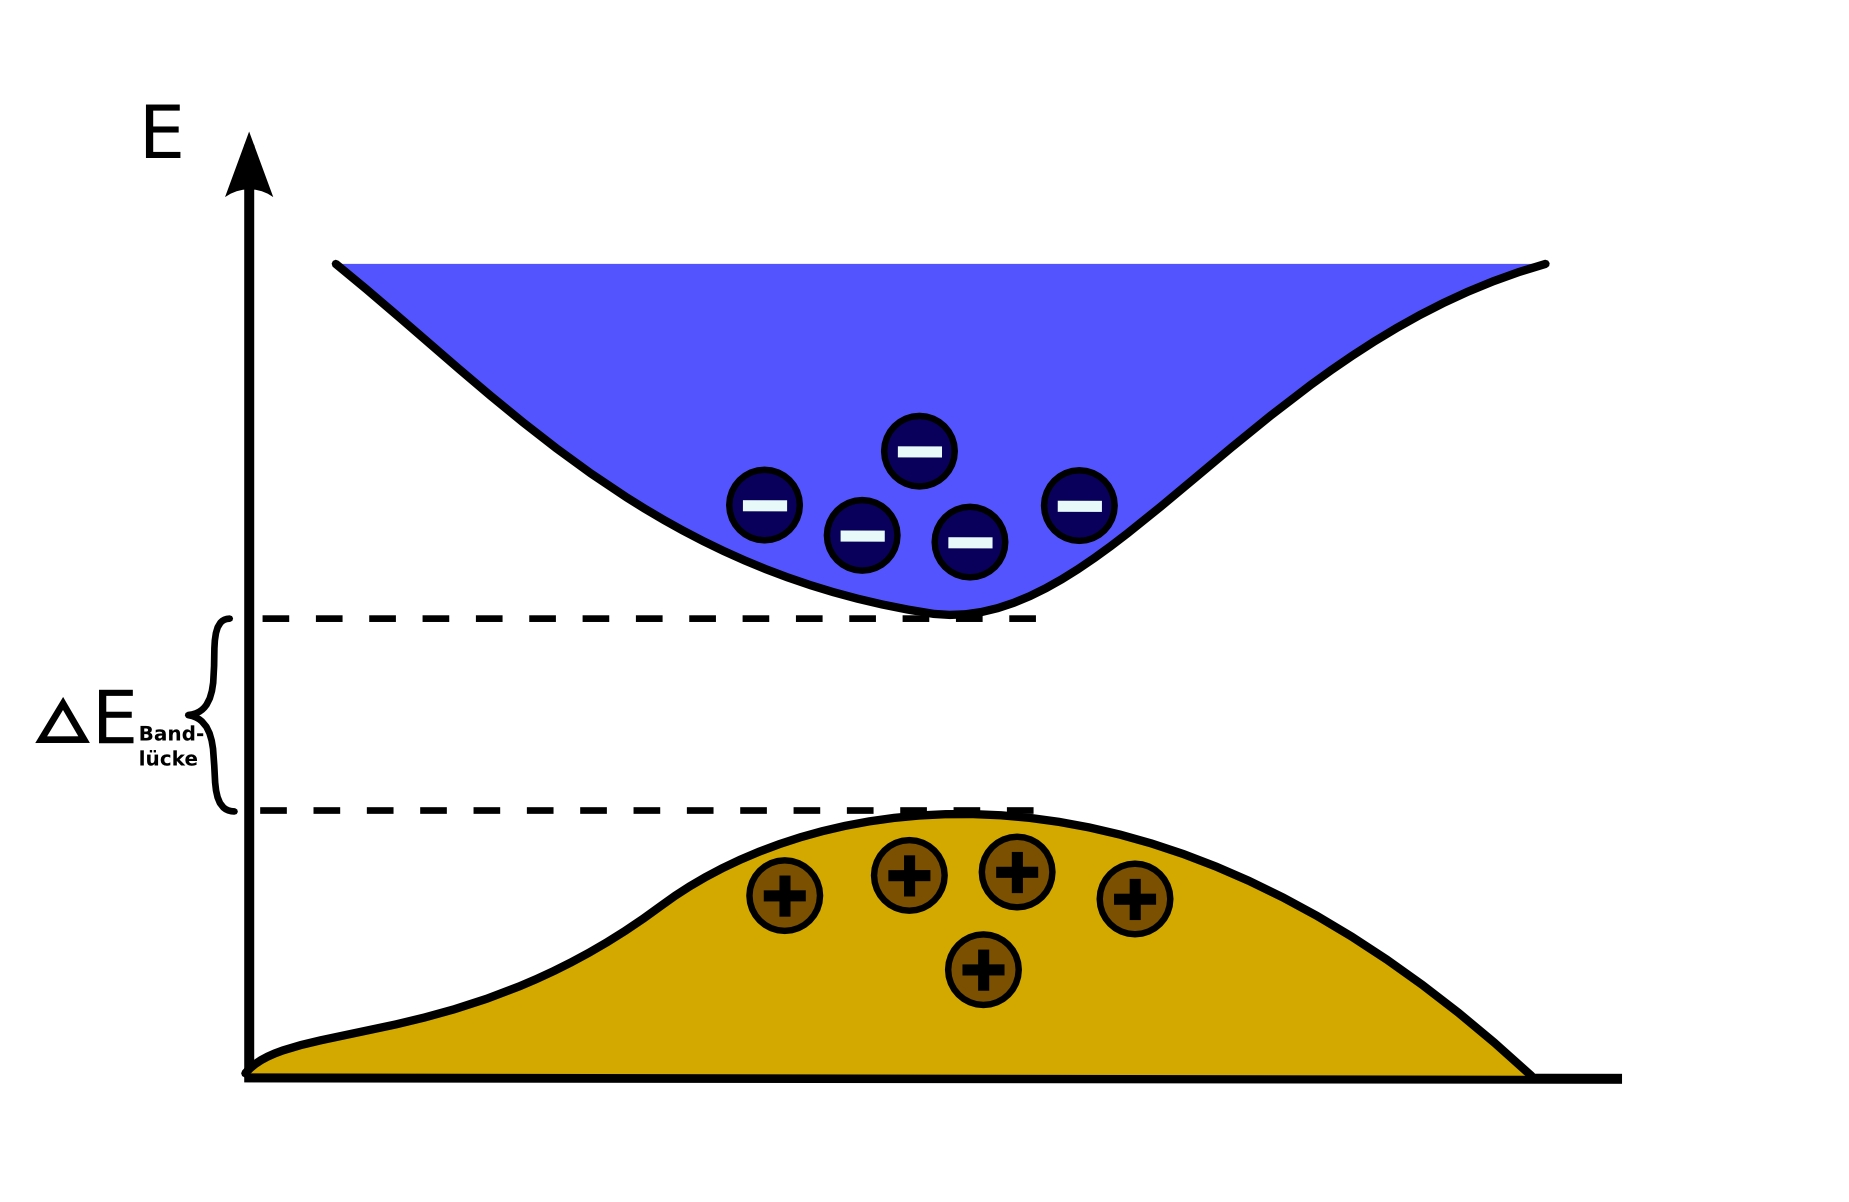
\includegraphics[width=0.8\textwidth]{images/band.jpg}
\end{center}
\vspace{-1.5\baselineskip}
\caption{Baenderstruktur der Halbleitergrenzschicht}
\label{Baendermodell}
\end{figure}

Die Energie dieses Photons entspricht der Bandlücke zwischen Valenzband und Leitungsband. Somit ergibt sich die Wellenlänge des emittierten Photons wie folgt:
 \[ \lambda = \frac{h \cdot c}{\Delta E_{\text{Bandlücke}}} \]
Dabei bezeichnet $h$ das Plancksche Wirkungsquatum und $c$ die Phasengeschwindigkeit des Lichts.

\subsection{Umkehrung des Effekts - LEDs in der Absorption}
In diesem Versuch sollten jedoch die LEDs nicht als Lichtemitter, sondern als Absorber dienen. Es wurde also versucht, die Funktionsweise der Lichtdioden umzukehren.

Bei Bestrahlung der LEDs mit Licht kann eine Spannung und ein Strom am Halbleiter abgegriffen werden. Besonderes Interesse gilt der Abhängigkeit dieses Stromes von der Wellenlänge des eingestrahlten Lichtes, je nach Farbe (Emissionswellenlänge) der LED. Da die Lichtdioden auch in der Absorption wellenlängenabhängig sind, ist es möglich aus mehreren Lichtdioden, die den gesamten visuellen Spektralbereich abdecken, ein Spektrometer für optische Spektren zu konstruieren.\\
Doch was passiert bei der Bestrahlung der LED durch Licht genügender Energie? Treffen Photonen auf die n-p-Grenzschicht des Halbleiterchips, werden dort Elektron-Loch-Paare erzeugt. Durch die Diffusionsspannung wandern die Elektronen in die p-dotierte Schicht, die positiven Löcher in die n-dotierte Zone, wodurch ein Stromfluss entsteht.

\subsection{Vergleich von Emissions- und Absorptionsspektren}
Es stellt sich jedoch die Frage, wie Absorptions- und Emissionsspektrum der Leuchtdiode zusammenh\"angen.
Es ist zu erwarten, dass die LED in der Absorption erst eine Spannung liefert, wenn die Energie der eingestrahlten Photonen mindestens dem Bandlückenabstand entspricht.
Tr\"agt man Absorptions- und Emissionskurve in einem Diagramm auf, ist gut zu erkennen, dass das Absorptionsspektrum gegen\"uber der Emission blauverschoben ist (\hypref{Abb.}{Absorption und Emission von LEDs}), und somit die LED erst auf das eingestrahlte Licht reagiert, wenn die Energie der Bandlücke weit überschritten ist. Quantitativ fällt die Verschiebung $\Delta \lambda$ bei verschiedenen LEDs jedoch unterschiedlich stark aus.
Ein konkreter Zusammenhang zur Wellenlänge der Leuchtdiode oder zum Halbleitermaterial konnte jedoch nicht gefunden werden.

\begin{figure}[ht]
\begin{center}
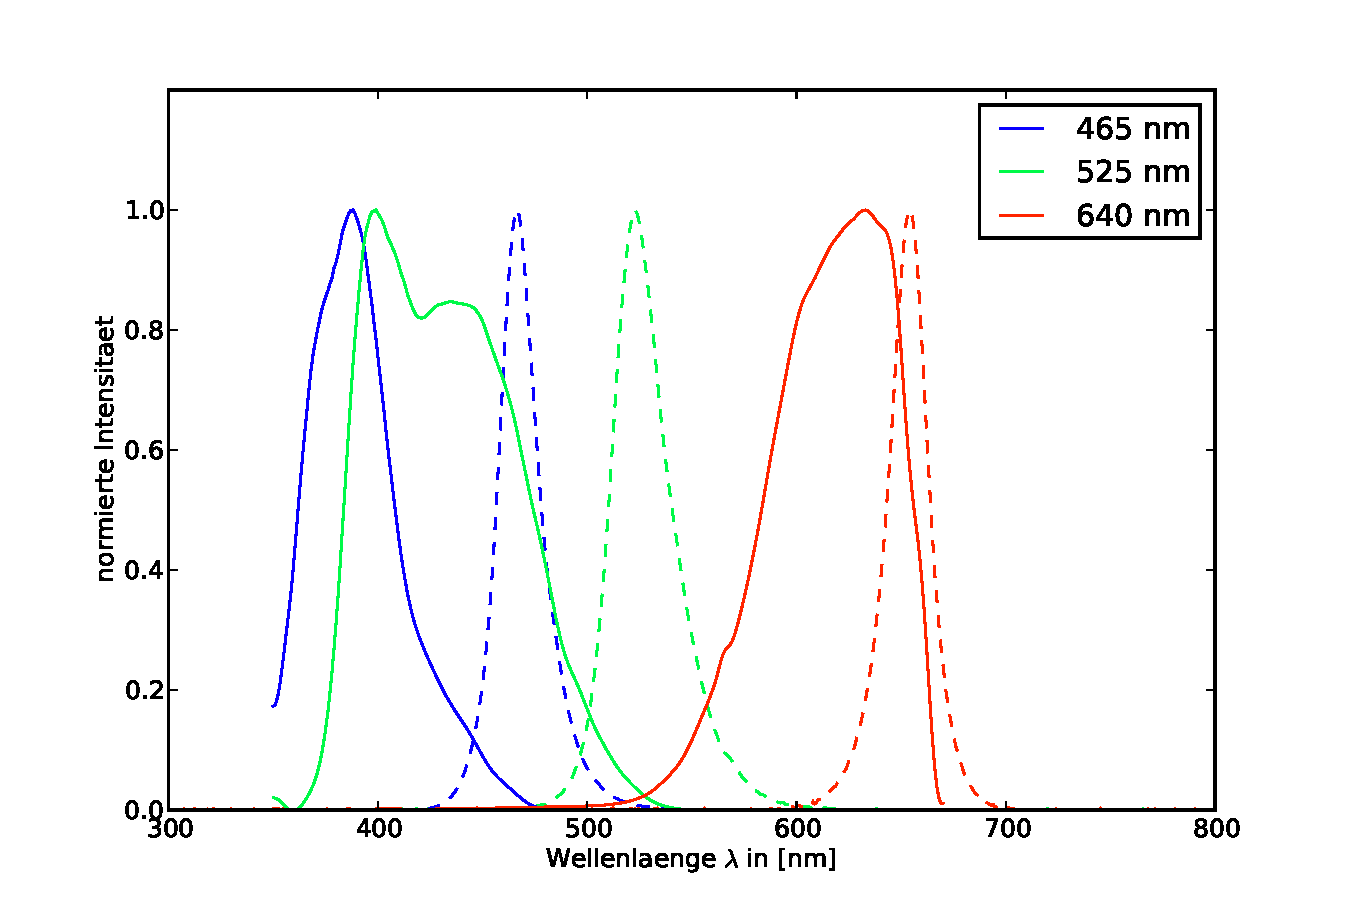
\includegraphics[width=0.9\textwidth]{images/absorp-emit.pdf}
\end{center}
\vspace{-1.5\baselineskip}
\caption{Absorptions- (durchgezogen) und Emissionsspektren (gestrichelt) verschiedener LEDs}
\label{Absorption und Emission von LEDs}
\end{figure}

%% Allg. was wir machen wollen, etwas Theorie 	Karl
%% Vergleich mit den Emissionsspekren}


\section{Messung der Absorptionsspektren}

\subsection{Versuchsaufbau}
%subsubsections wohl lieber weglassen, aber zur Meinungsbildung erst noch drinnen gelassen???	
\subsubsection{Lichtquelle} %%Axi
\begin{figure}[ht]
\begin{center}
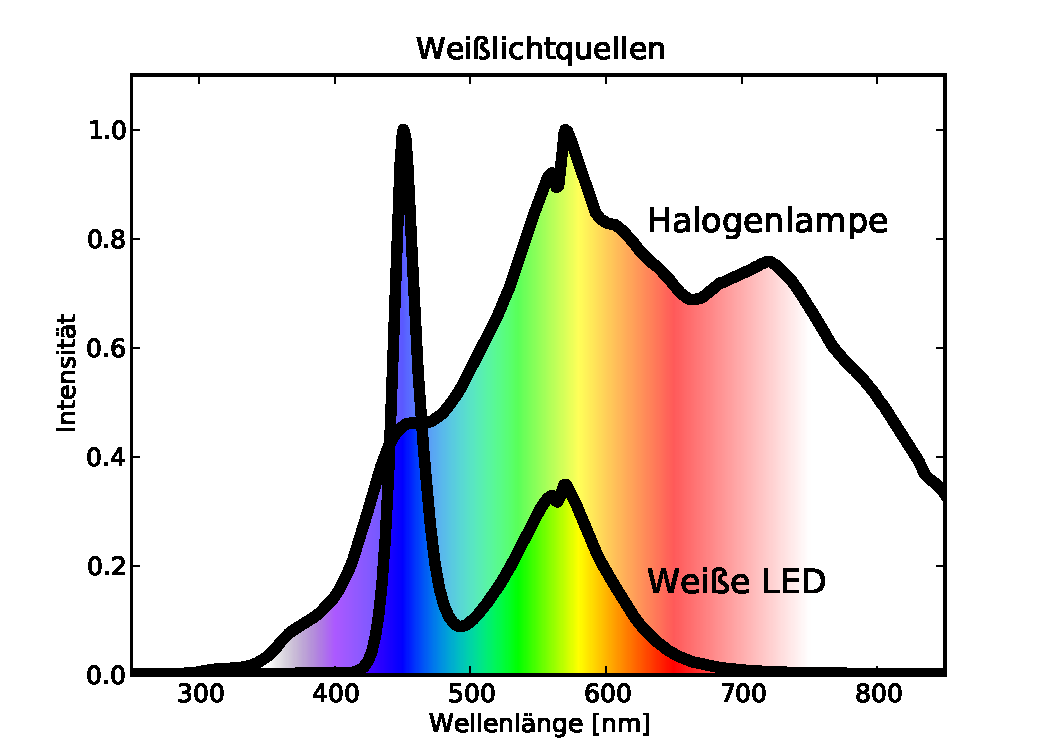
\includegraphics[width=1\textwidth]{images/quellspektren.pdf}
\end{center}
\vspace{-1.5\baselineskip}
\caption{Die beiden verwendeten Weißlichtquellen im Vergleich, gemessen mit dem professionellen Spektrometer der Optiker}
\label{fig:lichtquelle}
\end{figure}
Die gew\"ahlte Lichtquelle sollte ein m\"oglichst breites Spektrum mit bekannter Intensit\"atsverteilung aufweisen. Da nur wenige verl\"a\ss{}liche Angaben bez\"uglich des jeweiligen Spektrums der Lampen zu finden waren, wurde beschlo\ss{}en das Spektrum der Lichtquelle mit einem entsprechenden Ger\"at im Institut f\"ur Optik zu ermitteln.

Zun\"achst wurde ein Verbund von 4 wei\ss{}en LEDs, die mit einem L\"ufter gek\"uhlt werden, als Lichtquelle f\"ur die Absorptionsmessung der sp\"ateren Mess-LEDs gew\"ahlt. Als Ergebnis der vier im Quadrat angeordneten LEDs wei\ss{}t deren aufgef\"achertes Spektrum waagrechte, dunkle Streifen auf, die von den Bereichen zwischen den LEDs stammen. Bei der Messung mu\ss{}te deshalb darauf geachtet werden, dass diese Zonen geringerer Intensit\"at zun\"achst durch Defokussieren des Aufbaus mithilfe der eingebauten Linsen verkleinert wurden und anschlie\ss{}end die LEDs die verbleibenden Streifen nicht kreuzen. Dies h\"atte entsprechende Verringerungen in der Intensit\"at des Absorptionsspektrums zur Folge, welche die Messdaten verf\"alschen w\"urden.

Bei der Auswertung wurde festgestellt, da\ss{} die Weißlicht-LED Lichtquelle sehr wenig Intensit\"at im UV-Bereich emittiert (siehe \hypref{Abb.}{fig:lichtquelle}). F\"ur die weiteren Messungen diente deshalb eine 50W Halogenlampe ohne UV-Filter als Lichtquelle. Diese zeigte st\"arkere Intensit\"at im UV-Bereich. Trotz ihrer Nennstromstärke von $4\unit{A}$ brannte die Halogenlampe erst bei $5,3\unit{A}$ durch, so dass wir sie bei $4,7\unit{A}$ betrieben um möglichst viel Intensität auch noch im UV-Bereich zu erhalten. Da die Halogenlampe durchaus Temperaturen um $200\cel$ erreichen kann, war eine gute Bel\"uftung und ausreichender Abstand hitzeempfindlicher Teile auch hier wichtig.

Im Plot der Weißlichtspektren wird neben der erwarteten Intensitätsverteilung auch eine Charakteristik des Spektrometers der Optiker erkennbar, wie z.B. die Delle bei $564\unit{nm}$. Dies ist ein Problem für spätere Kalibrierungen mit diesem Spektrum, da wir eigentlich davon ausgegangen sind dass es die Spektren unverfälscht wiedergibt.

\subsubsection{Strahlengang und Messaufbau} %%optischer Strahlengang ist unten eingebaut. Deshalb auch die Idee, die subsubsections weg zu lassen.
Zur Erzeugung eines Spektrums gibt es diverse M\"oglichkeiten. Es stellte sich aber heraus, dass die Verwendung eines Prismas aufgrund der geringen Winkelausdehnung des erzeugten Spektrums f\"ur uns wenig lohnenswert ist. Ebenso mussten wir trotz langen Experimentierens und unter Verwendung verschiedener Linsenanordnungen auch auf ein Transmissionsgitter verzichten, da die Intensit\"at des Spektrums nicht stark genug war. Folglich griffen wir auf ein holographisches Reflexionsgitter zur\"uck, welches mit einer Gitterkonstanten von $d=2400\unit{\text{Linien}/mm}$ ein sehr breites Spektrum erzeugt .%%Gitterkonstante und Winkelausdehnung des Spektrums angeben 2400/mm

%%\subsubsection{Winkelmessung} %%--- Eher "Wellenl\"angenbestimmung" oder dergleichen?! Da wir dadurch ja die momentan gemessene Wellenl\"ange bestimmen m\"ochten
F\"ur die Auswertung der Messdaten ist es von grundlegender Bedeutung, zu wissen welcher Wellenl\"ange die gemessene Intensit\"at zuzuordnen ist. Um dies zu erreichen wurde folgendes Vorgehen gew\"ahlt: Durch die Verwendung eines Refelxionsgitters und dessen Justierung derart, dass der Strahlengang in einer zum optischen Tisch parallelen Ebene verl\"auft, l\"asst sich die Wellenl\"ange durch \hypref{Formel}{eq:gitter} leicht in den Winkel zwischen ein- und ausfallendem Strahl $\alpha$ umrechnen mit dem Drehwinkel des Gitters $\varphi = 65,8\degr$.
\begin{equation}
\frac{\lambda}{d} = \sin(\varphi) - \sin(\alpha + \varphi)
\label{eq:gitter}
\end{equation}
Da ein manuelles Auslesen der Intensit\"at und dessen zugeh\"origem Winkel ein aussichtsloses Unterfangen darstellen w\"urde, benutzten wir ein Drehpotentiometer zur automatischen Auswertung des momentanen Winkels. Dieses wurde so auf dem Tisch positioniert, dass die Drehachse m\"oglichst genau unter dem Mittelpunkt des Gitters ist, also dem Punkt, an welchem sich ein- und ausfallender Strahl treffen. Desweiteren wurde der Dreharm, an dessen \"Au\ss{}erstem Ende sich der Halter f\"ur die LEDs befindet, mit der Drehachse verbunden, sodass das Schwenken des Armes den Widerstand des Potentiometeres \"andert.
\begin{figure}[ht]
\begin{center}
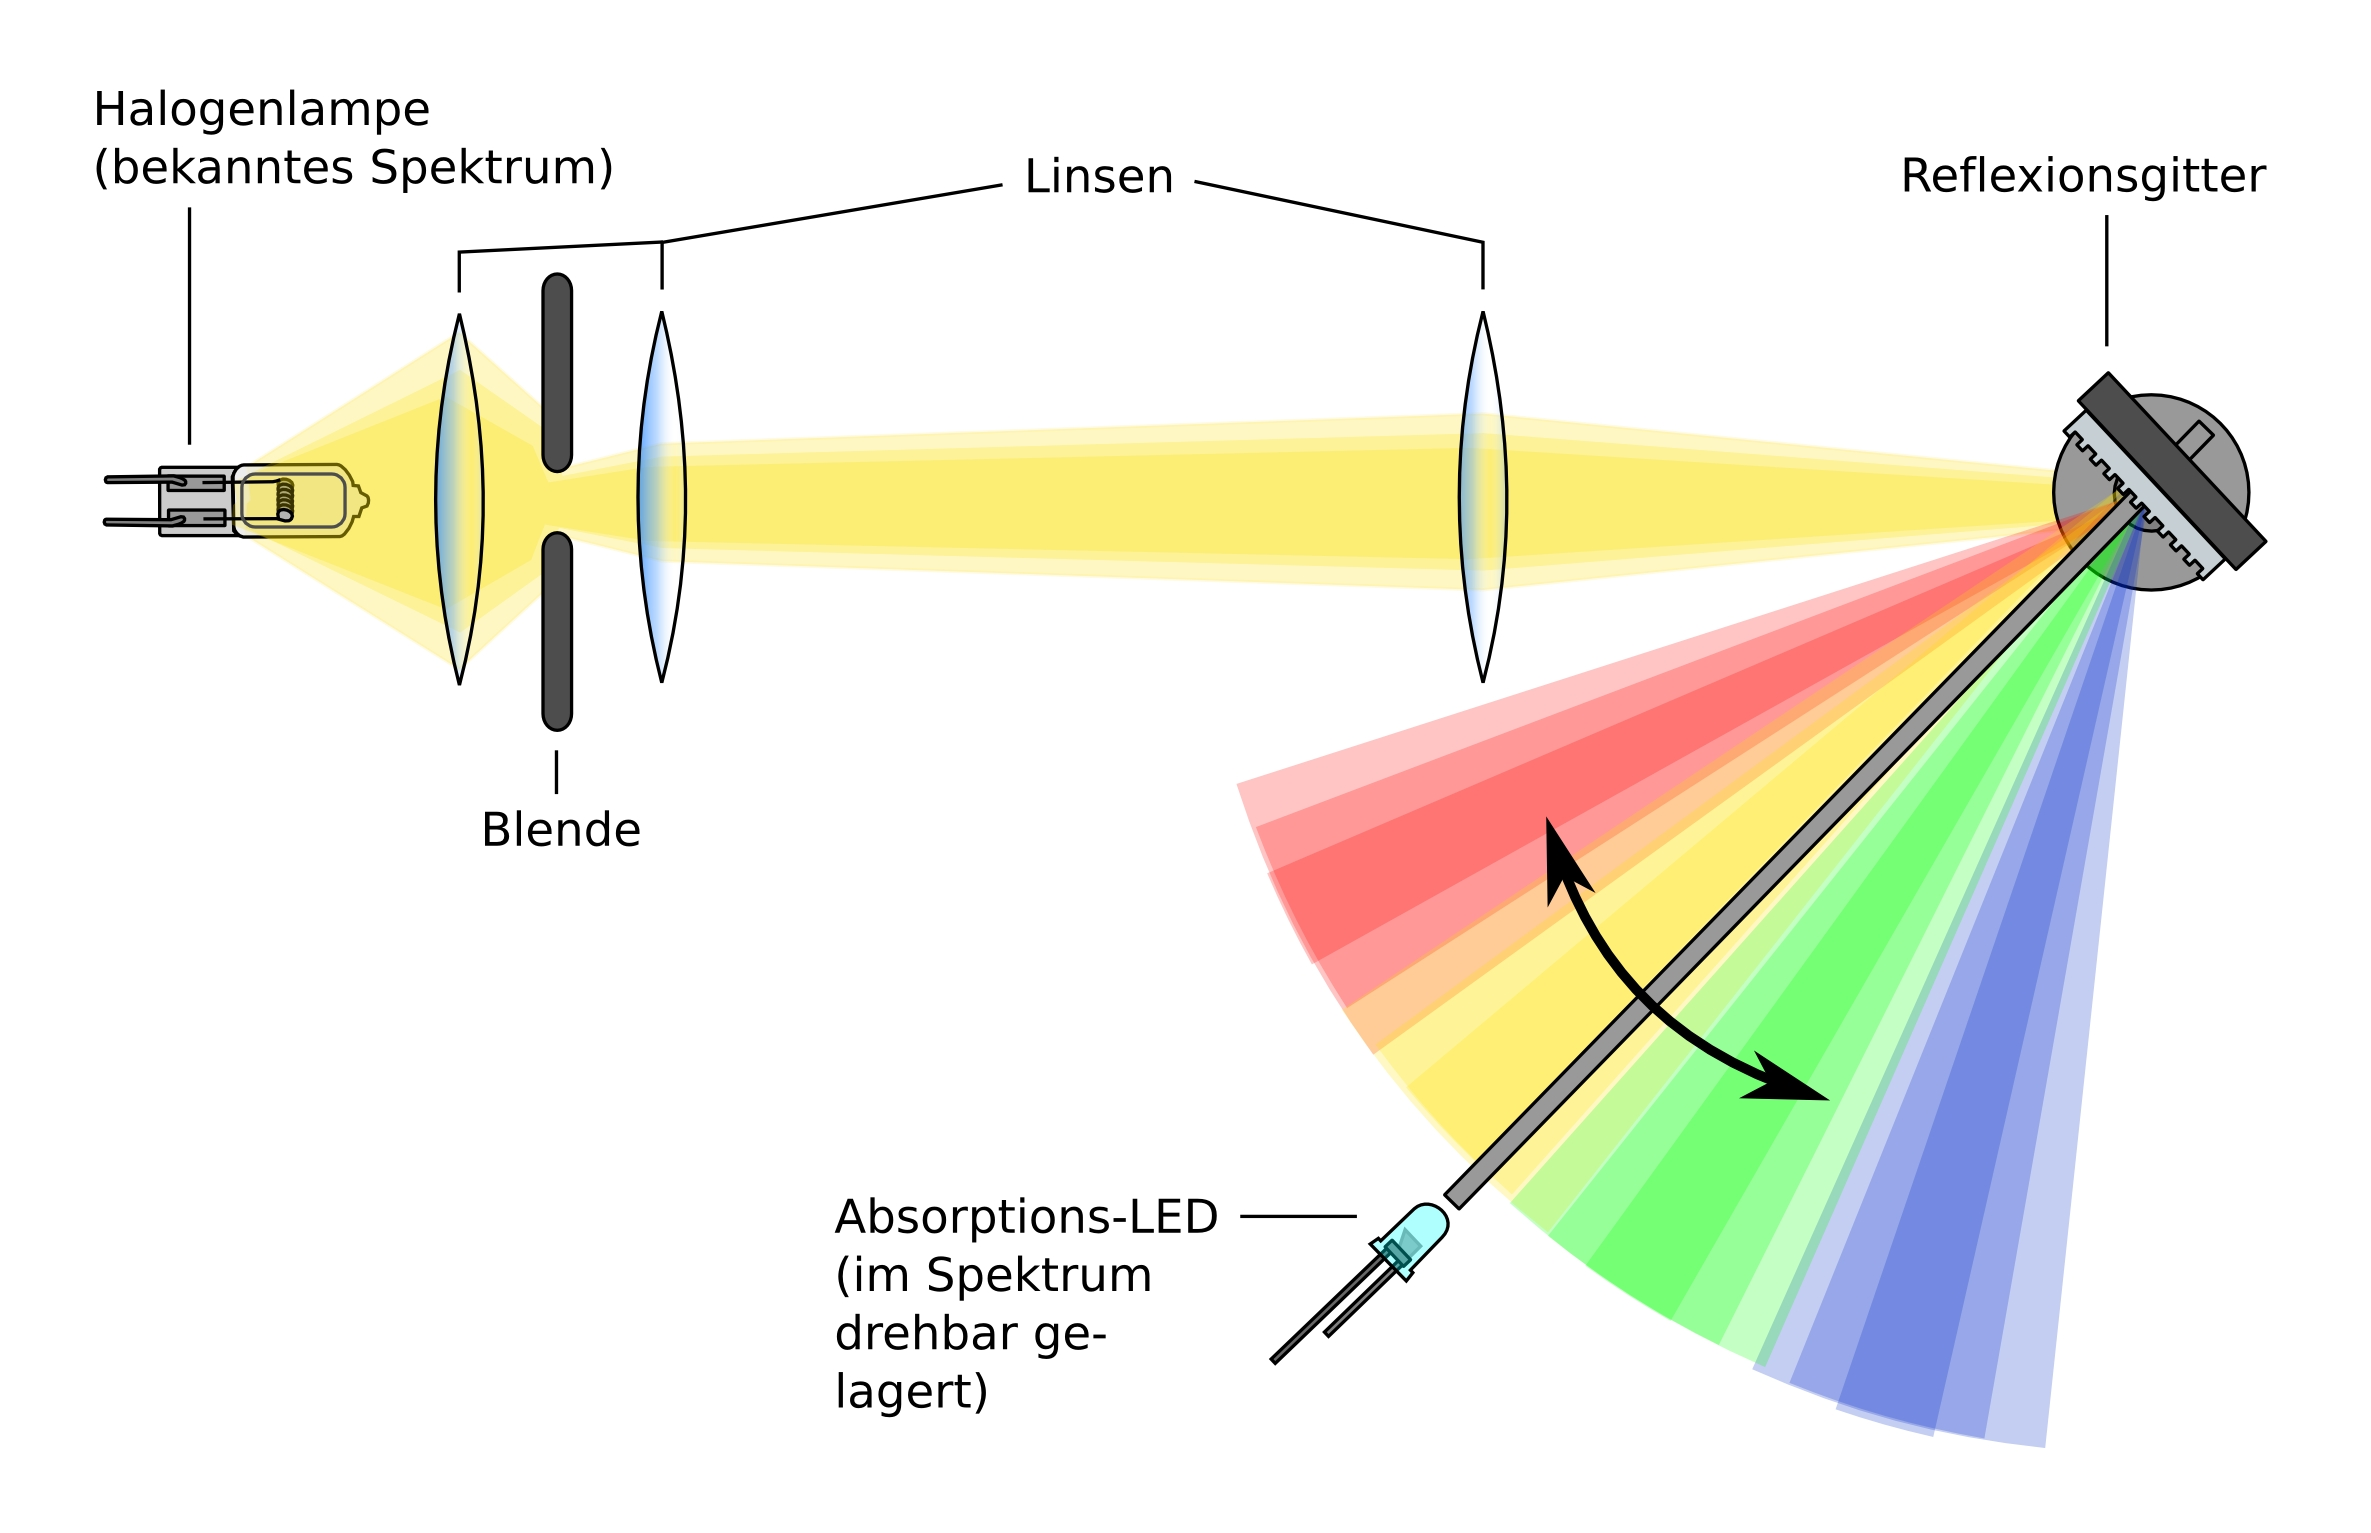
\includegraphics[width=0.8\textwidth]{images/setup.jpg}
\end{center}
\vspace{-1.5\baselineskip}
\caption{Versuchsaufbau}
\label{Versuchsaufbau}
\end{figure}

Anschließen wurde in $2^\circ$-Intervallen der Winkel und die Spannung am Potentiometer notiert. Wiederholtes Messen dieser Spannungs-Winkel-Abhängigkeit zeigte eine sehr gut Reproduzierbarkeit. Lediglich beim Wechsel des Drehsinns zeigte sich ein Offset, so dass entschlossen wurde alle Messungen immer mit Drehung im Uhrzeigersinn durchzuführen.

Somit konnten wir die momentane Spannung am Potentiometer auslesen lassen, was uns den Winkel gibt und somit die Wellenlänge berechnen lässt.
\begin{figure}[ht]
\begin{center}
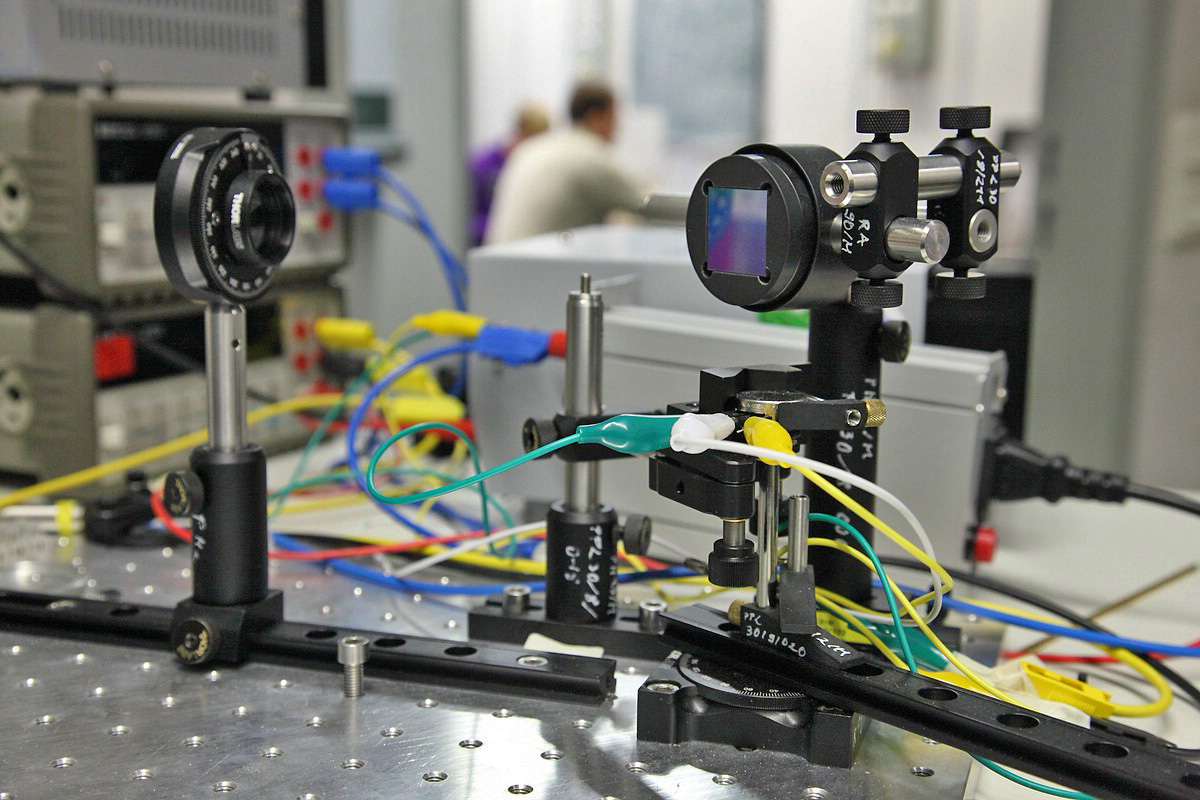
\includegraphics[width=0.8\textwidth]{images/poti-reflexgitter.jpg}
\end{center}
\vspace{-1.5\baselineskip}
\caption{Das Reflexionsgitter zur Erzeugung des Spektrums und das Potentiometer zur Winkelmessung}
\label{winkel_spannung}
\end{figure}

\begin{figure}[ht]
\begin{center}
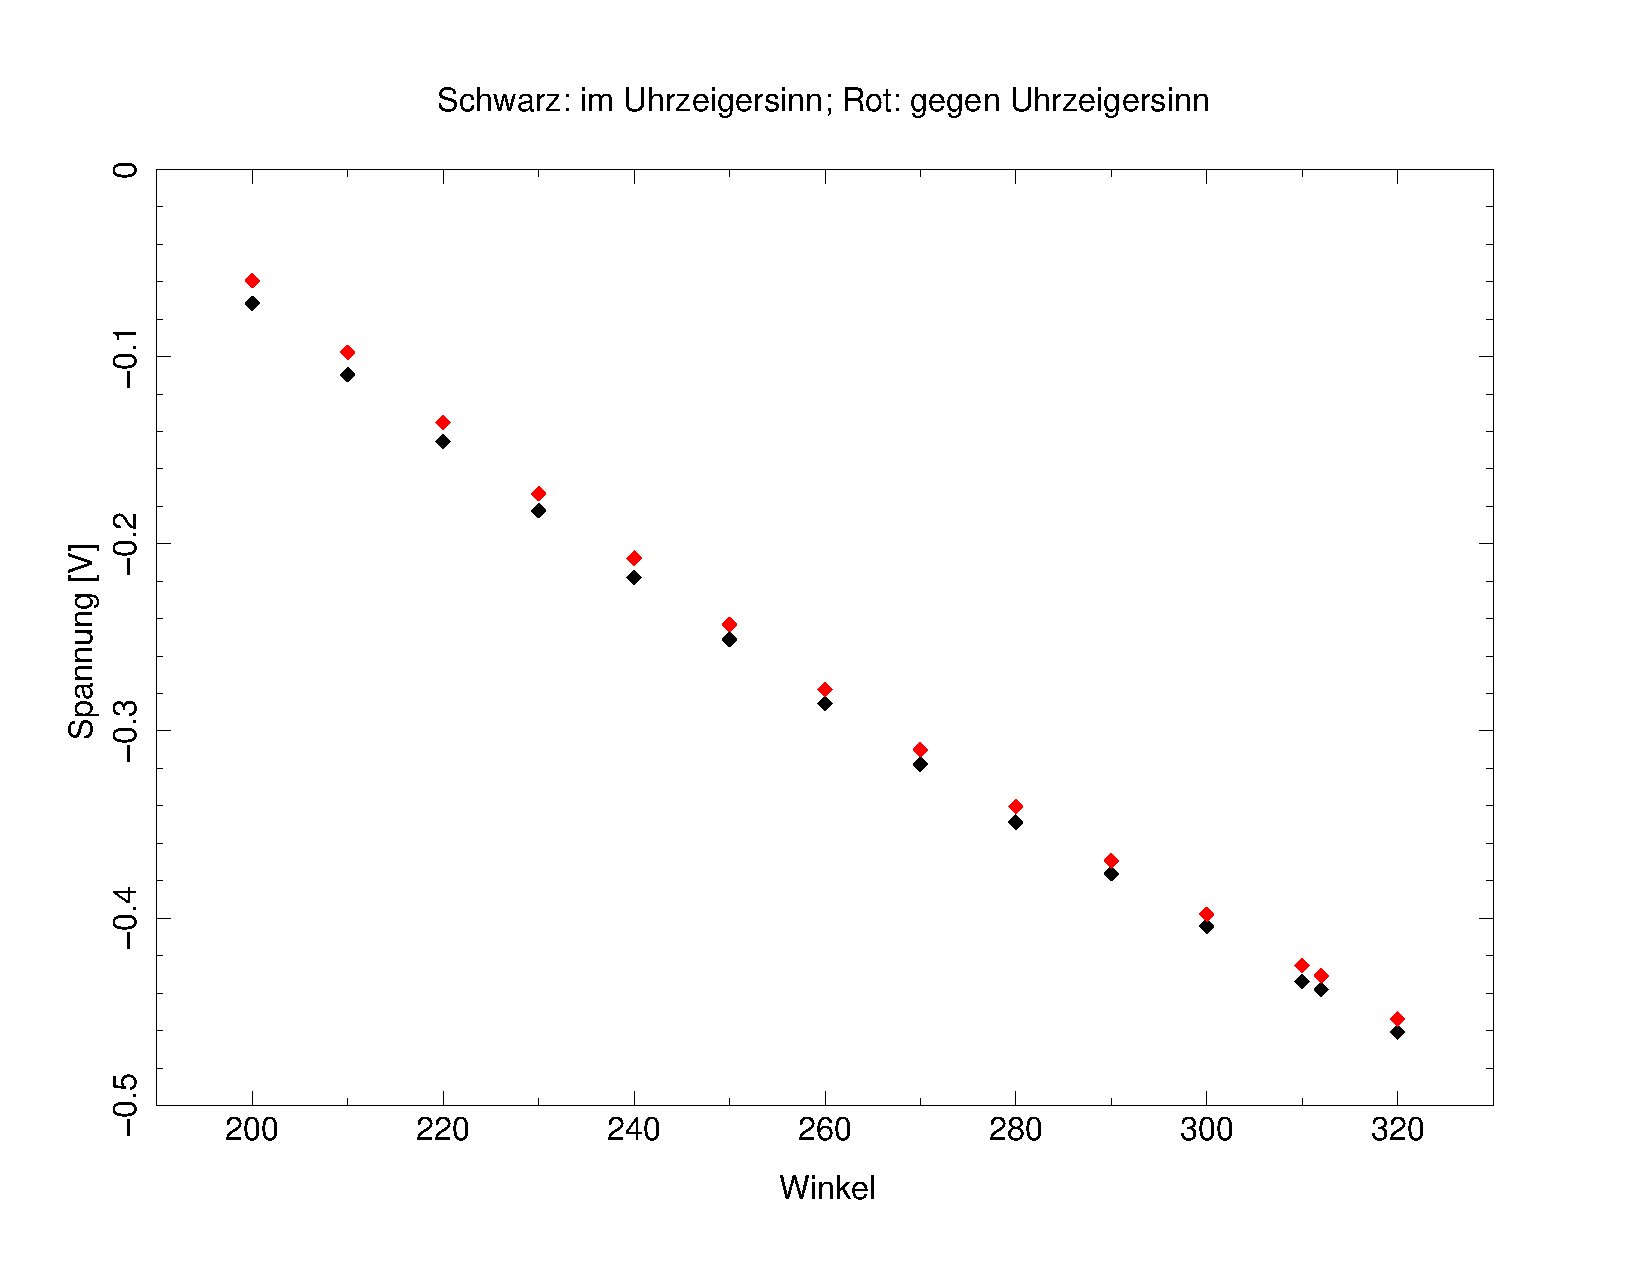
\includegraphics[width=0.8\textwidth]{images/winkel_spannung_grob.pdf}
\end{center}
\vspace{-1.5\baselineskip}
\caption{Die Potentiometerspannung in Abhängigkeit vom Drehwinkel}
\label{winkel_spannung}
\end{figure}


\subsection{Reduktion der Spektren}
Aus den aufgenommenen Rohdaten konnten wir mit Hilfe eines hierzu erstellten 500-Zeilen Python Skripts die benötigten Spektren $I(\lambda)$ berechnen.
Die elektronisch per Computer gemessenen Daten waren Wertepaare von Potentiometerspannung und Absorptions-LED Spannung über einen Lastwiderstand von $100\unit{k\Omega}$.

Als ersten Schritt wurden die Potentiometerspannungen mit Hilfe der in \hypref{Abb.}{winkel_spannung} gefundenen invertierbaren Funktion in Drehwinkel umgerechnet.
Der Winkelbereich des optischen Spektrums lag zwischen $111\degr$ und $158\degr$ (siehe \hypref{Abb.}{Versuchsaufbau}), wo wir die Potentiometercharakteristik sehr gut vermessen hatten.
Als nächstes wurden die Winkel mit Hilfe von \hypref{Gleichung}{eq:gitter} in Wellenlängen umgerechnet. Da der Drehwinkel $\varphi$ des Gitters allerdings schwierig zu messen war, wurde das Interferenzmaximum erster Ordnung, bei dem sich das Gitter wie ein Spiegel verhält, mit aufgezeichnet und aus dessen Lage in der Software der Drehwinkel ausgerechnet. Zusätzlich mussten die Intensitätswerte nach dem Transformationssatz skaliert werden, weil die Wellenlängen nicht gleichmäßig über den Winkelbereich verteilt sind:
\begin{equation}
I(\lambda) = I(\alpha(\lambda)) \;/\; \frac{\dif\lambda}{\dif\alpha}
\end{equation}

\subsubsection{Entfaltung der Spektren}
Im nächsten Schritt wurde versucht, die Spektren zu entfalten.
Unsere Lichtquelle war natürlich keine Punktquelle und mit dem Linsensystem gelang es auch nicht, die Glühlampe auf einen sehr kleinen Punkt abzubilden.
Infolgedessen würde eine scharfe Spektrallinie als verwaschener Peak erscheinen und von der Absorptions-LED entsprechend aufgenommen werden. Unser gesamtes Spektrum wird somit etwas verbreitert und unscharf gemacht.
Mathematisch gesehen ist das eine Faltung und zwar mit der Punktantwort des optischen Systems als Faltungskern.
Unser Ziel war es also, diese Operation rückgängig zu machen, also eine Entfaltung der Spektren durchzuführen.

Die Punktantwort des Systems konnte relativ einfach bestimmt werden, indem die Intensitätsverteilung um das 0. Interferenzmaximum herum gemessen wurde.
Die Entfaltung selbst ist jedoch eine relativ schwierige Operation, da nicht unbedingt eine eindeutige Lösung existiert, und kleine Fehler im Signal überinterpretiert und zu großen Fehlern in der Lösung führen können.

Somit haben wir verschiedene Algorithmen ausprobiert und auf ihre Tauglichkeit überprüft.
Ein vielversprechender Ansatz war die "`Wiener Deconvolution"'.
Diese nutzt aus, dass die Faltung im Fourierraum einer Multiplikation entspricht, wodurch man zum Entfalten eine Division im Fourierraum durchführen muss.
Zur Unterdrückung von zu starken Rauscheffekten geht noch eine Abschätzung der Fehler im jeweiligen Frequenzbereich mit ein.
Leider mussten wir aber feststellen, dass das Verfahren insgesamt nicht die erwünschten Ergebnisse liefern konnte, vor allem weil die verschiedenen Frequenzterme sich immer auf das ganze Spektrum auswirken.
Das Glätten von Oszillationen an einer Stelle führte gleichzeitig auch zu Verfälschungen an spitzen Peaks.

\begin{figure}[H]
\begin{center}
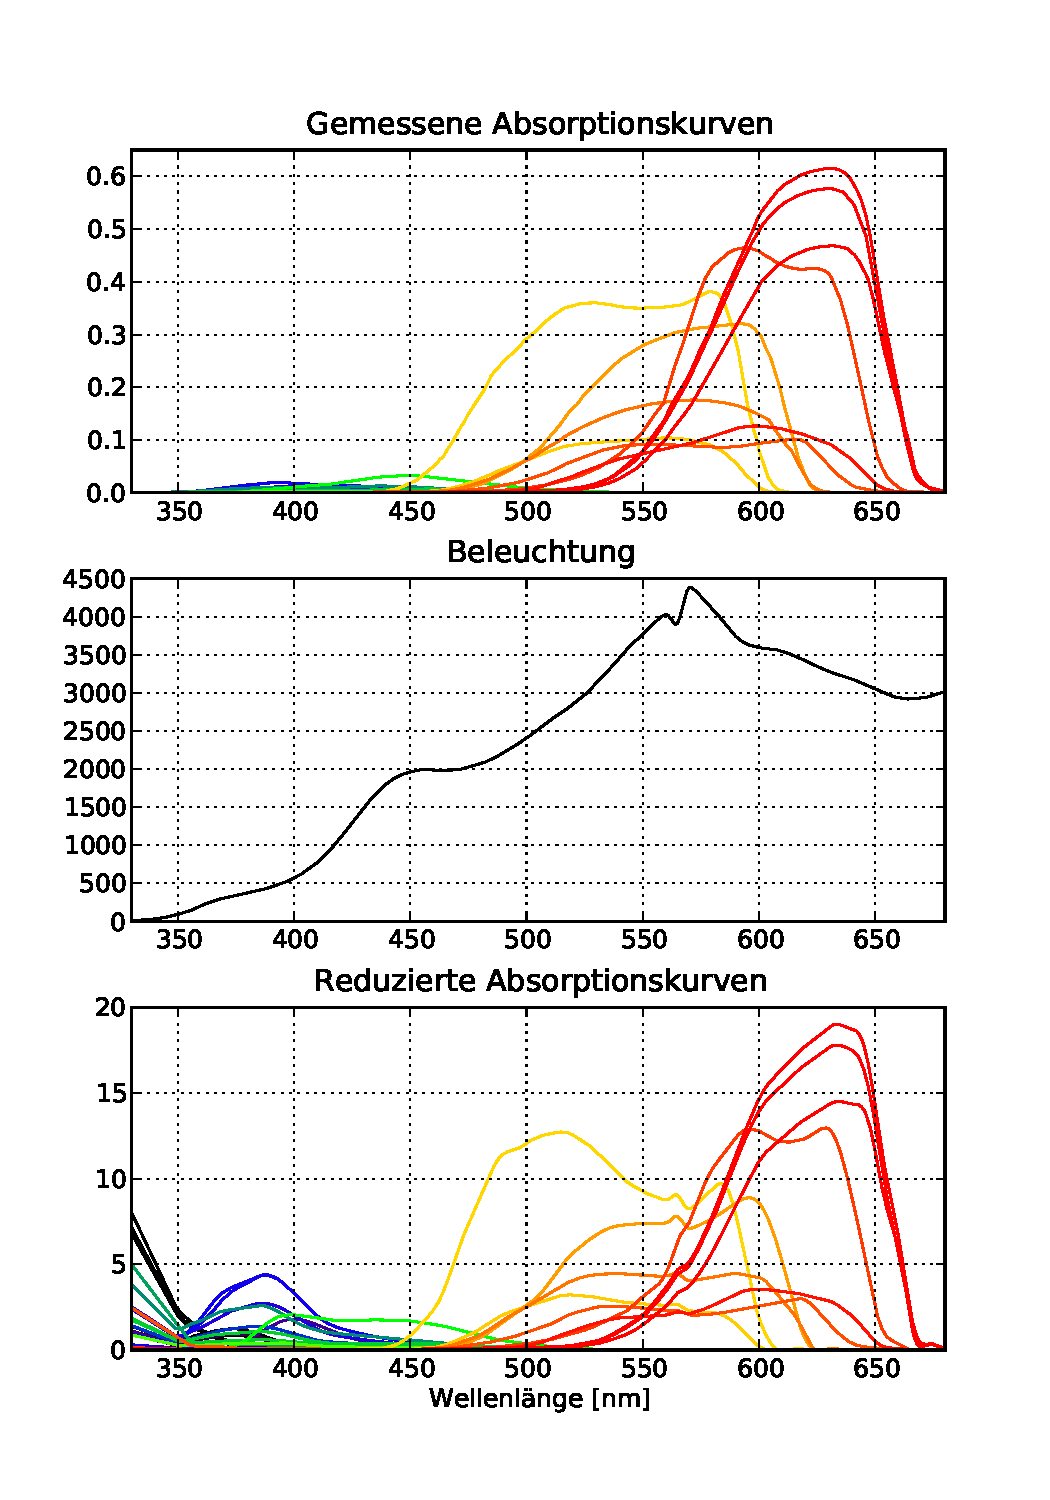
\includegraphics[width=1\textwidth]{images/spektren_mit_halogen.pdf}
\end{center}
\vspace{-1.5\baselineskip}
\caption{Reduktion der gemessenen LED-Absorptionsspektren}
\label{fig:reduktion}
\end{figure}
Der zweite Ansatz führte auf Matrizen.
Da wir ohnehin auf diskretisierten Daten arbeiten, kann man die Faltung auch als Matrix-Multiplikation interpretieren.
Die Entfaltung entspricht dann einer Invertierung.
Die direkte Invertierung ist aber wieder völlig unbrauchbar, da extrem starke Oszillationen entstehen.
In der Tat wären diese eine Lösung des Entfaltungsproblems, nur eben nicht die gesuchte.
Zur Unterdrückung der Oszillationen haben wir nun die Methode der kleinsten Quadrate instrumentalisiert.
Nach dem bekannten Trick, an ein Matrixgleichungssystem einfach von links die transponierte Matrix anzumultiplizieren kann man noch zusätzliche Terme hinzuaddieren, die dann bei der Lösung des Systems mit minimiert werden.
In diesem Fall addiert man die Matrix, welche für jeden $x$-Wert die Krümmung ausrechnet, so dass das System wie folgt aussieht:
\begin{equation}
(A^t A + K^t K)\cdot x = A^t\cdot b
\qquad\qquad
K = \alpha\cdot
\begin{pmatrix} 
  1 &	-2 &	1 &	&	\\
  &	\ddots&	\ddots&	\ddots&	\\
  &	&	1 &	-2 &	1
\end{pmatrix} 
\end{equation}
Hierbei ist $A$ die Faltungsmatrix, die aufgrund der endlichen Faltungsbreite eine Bandstruktur aufweist, $K$ die Krümmungsmatrix mit einstellbarem Vorfaktor $\alpha$, $b$ das gemessene Spektrum und $x$ die Lösung des entfalteten Spektrums.
Die so erzeugten Lösungen erschienen relativ brauchbar.
Anstatt von $K$ wurden auch Matrizen probiert, die auf Terme höherer Ordnung reagieren, was aber zu keinem signifikant besserem Ergebnis geführt hat.
Nachteilig an so einem linearen Verfahren ist natürlich, dass negative Lösungen an einigen Stellen nicht unterdrückt werden können.

Am Ende zeigte sich, dass die Absorptionsspektren relativ breit sind im Vergleich zum Faltungskern.
Der Effekt der Faltung ist also relativ gering wenn man bedenkt dass dieser auch nur an Stellen auftritt, wo die Funktion gekrümmt ist.
Letztlich wäre es also kein großer Fehler gewesen, die Faltung komplett zu vernachlässigen und die Spektren ohne Entfaltung zu übernehmen.

Zwischen den einzelnen Schritten mussten die Daten für manche Operationen auf ein äquidistantes Gitter gebinnt werden, was einfach mit linearer Interpolation durchgeführt wurde.
Als letzten Schritt wurde berücksichtigt, dass das eingestrahlte Spektrum nicht gleichhell in allen Wellenlängen war.
Die Spektren wurden nun einfach noch durch die Intensität der jeweiligen Lichtquelle (\hypref{Abb.}{fig:lichtquelle}) geteilt.
Am Rand des Spektralbereichs, wo die Intensität gering war, sieht man daher auch die größten Fehler.
Weiterhin fällt auf, dass die gemessenen Lichquellen ein bestimmtes Muster enthalten, was bei unseren Messungen aber nicht vorhanden war, und daher invers aufgeprägt wurde.
Dieser Fehler kann fast nur an dem kommerziellen Kalibrations\-spektrometer liegen.

Die Fertig reduzierten Absorptions\-spektren sind in \hypref{Abb.}{fig:reduktion} dargestellt.



\section{Bau des Spektrometers}
\subsection{Funktionsprinzip Übersicht}

\subsection{Elektronik}
%% Funktionsprinzip OpAmps etc.			Michele, Maria
%% Schaltplan

\subsection{Auswertungsprogramm}
% Software: Berechnung der Spektren mit unserem Gerät
%% Funktionsübersicht und Erklärung der Bedienung
%% Algorithmik zur Auswertung					BAsti



\newpage
\section{Autorenverzeichnis}
\begin{tabular}{|l|l|}
\hline
\emph{Autor} & \emph{Kapitel}\\
\hline
Michele Collodo & \\
Andreas Glossner & \\
Karl-Christoph G\"odel & \\
Bastian Hacker & \\
Maria Obst & \\
Alexander Wagner & \\
David Winnekens &  \\
Wickie Pedia & Recherchen \\
\hline
\end{tabular}
\end{document}

